\section{Myo armband overview}

The Myo armband from Thalmic Labs will be used for EMG data acquisition. It contains 8 dry stainless steel electrode-pairs around the inside of the armband, as depicted in \figref{fig:myoarmband}. The recorded EMG is unitless and in 8-bit resolution, and therefore not represented in volts as EMG normally is. But as usual EMG the higher the performed contraction is, the higher the integer values in the output will be. To avoid interference from the power lines a 50 Hz notch filter is implemented in the Myo armband. The Myo armband is not able to make any further filtering, and will thus be implemented digitally later in the signal processing. The Myo armband pulls the data with a 200 Hz sample rate. Besides the EMG sensors the Myo armband contains a nine axis inertial measurement unit consisting of three axis gyroscope, three axis magnetometer and three axis accelerometer. This inertial information is pulled at a 50 Hz sample rate. The inertial measurement units gives information about the orientation, position and movement of the user’s arm. 

\begin{figure}[H]                 
	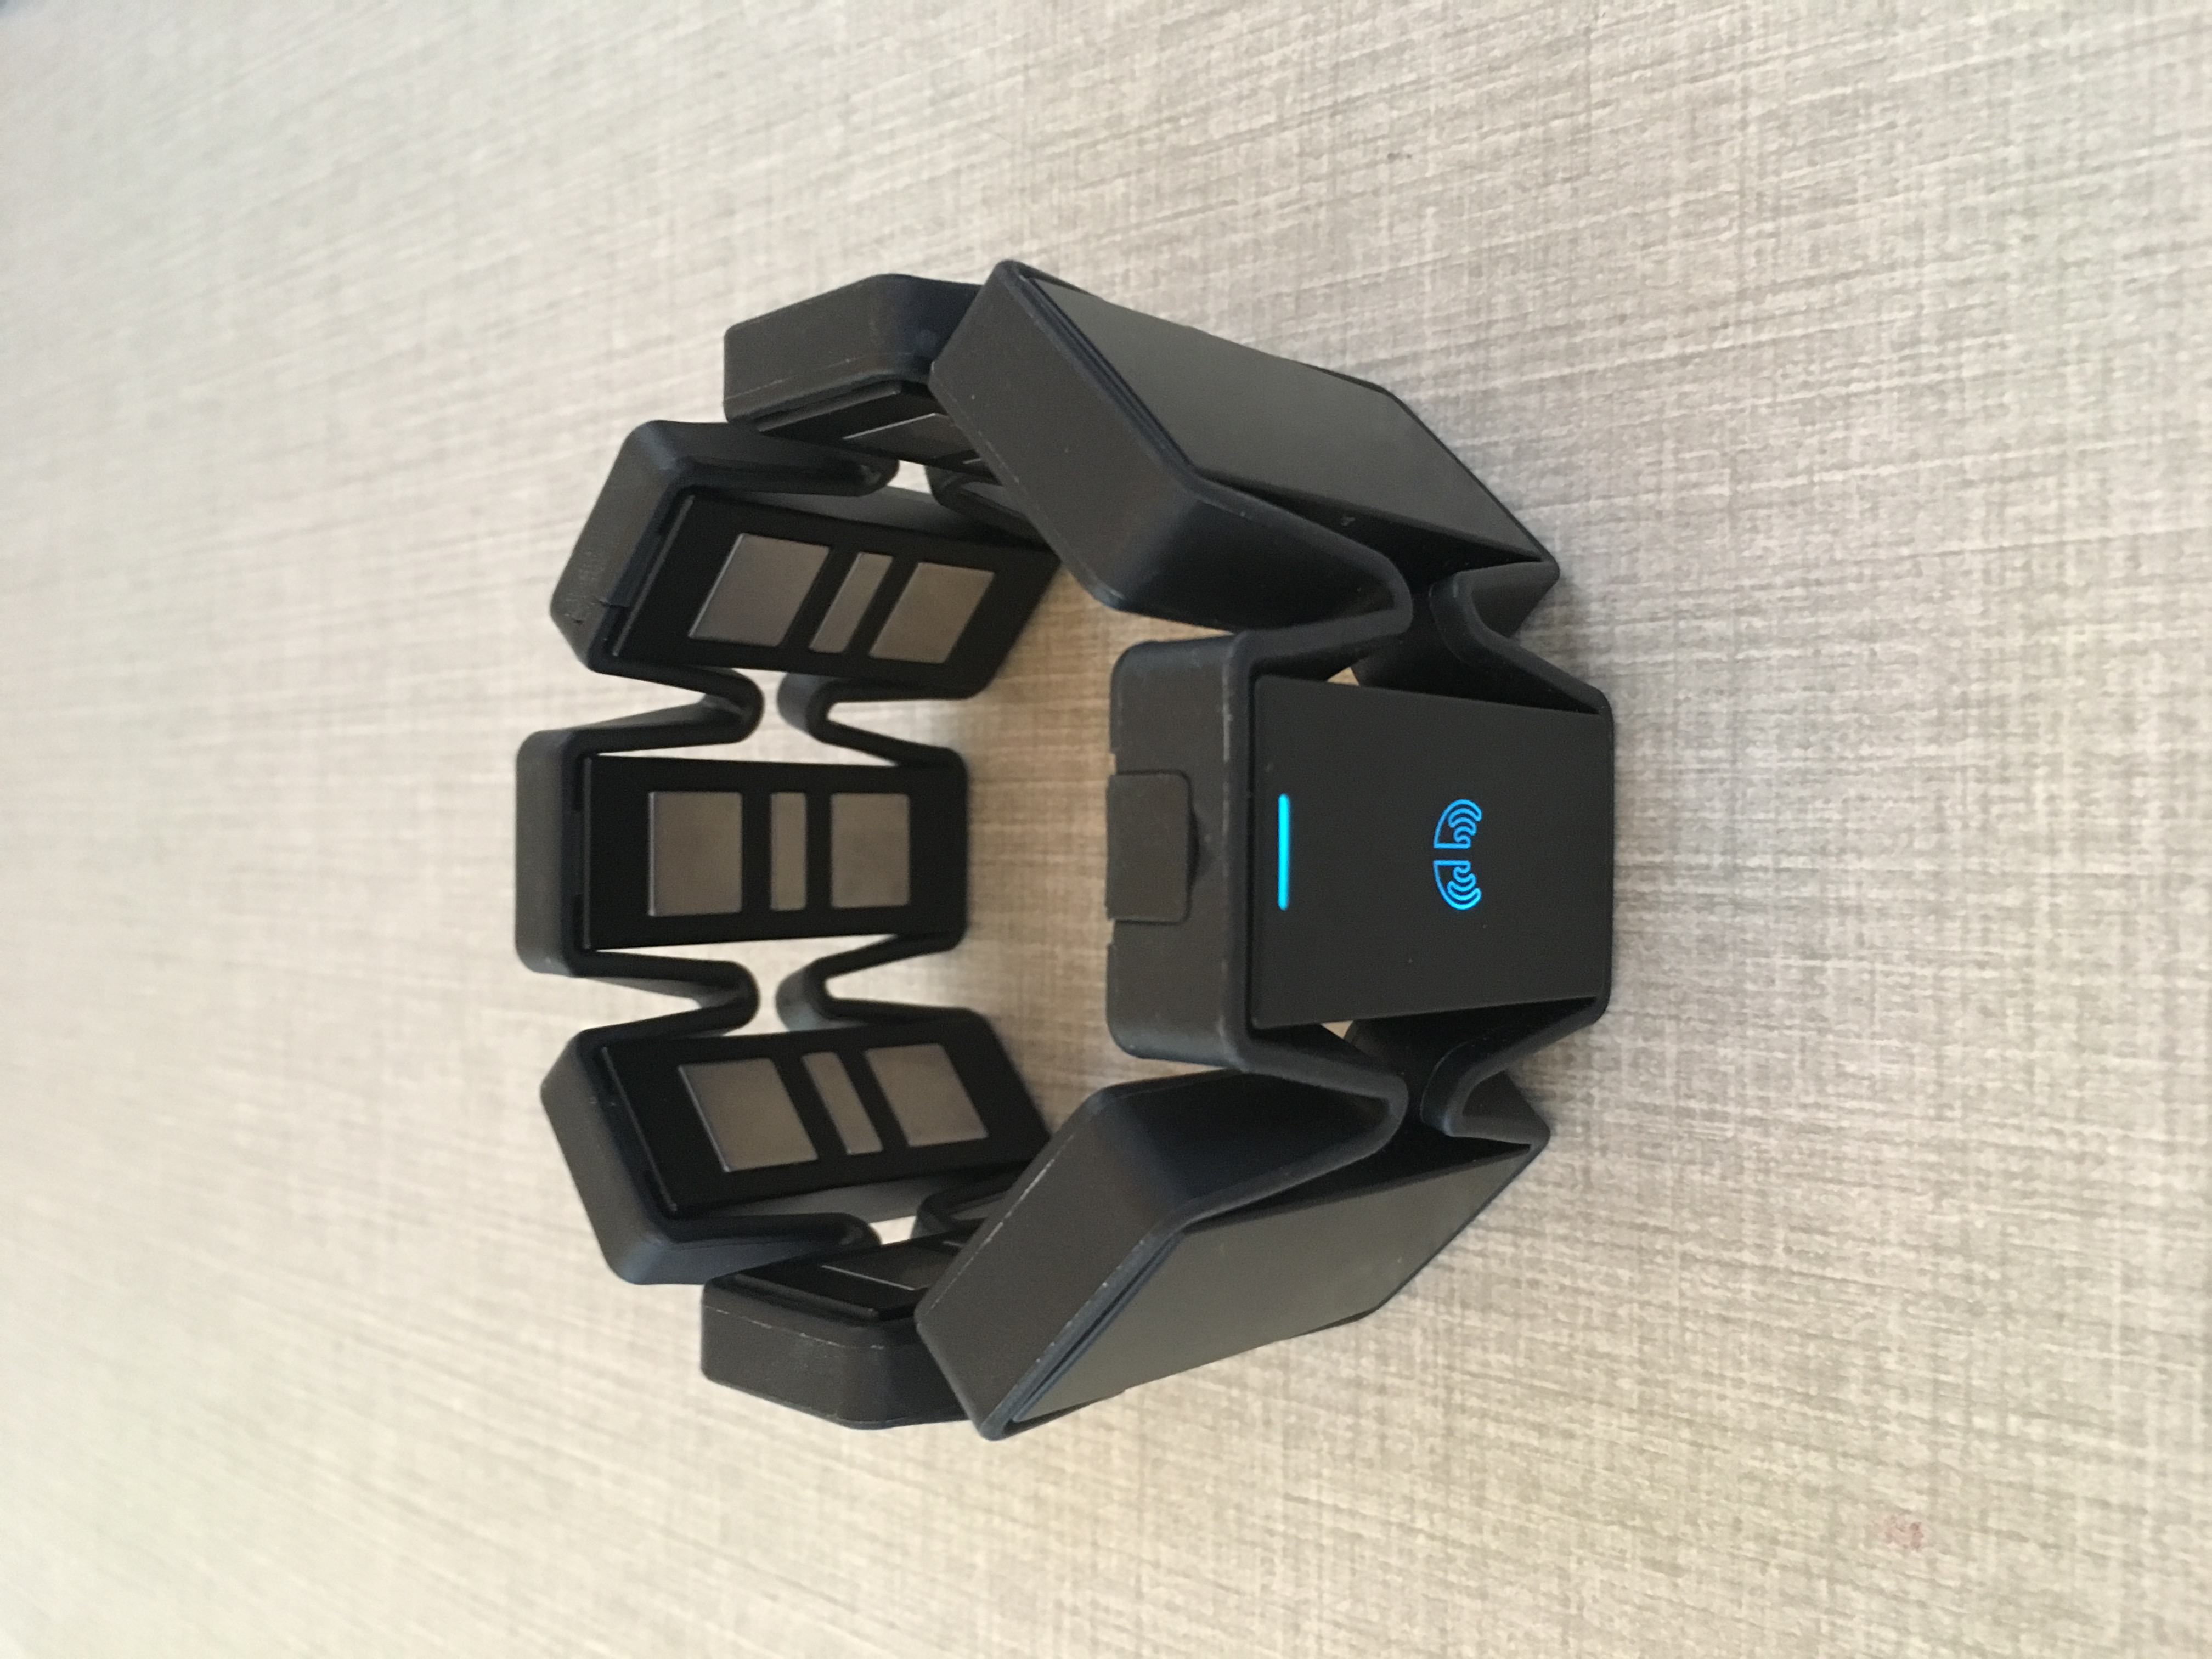
\includegraphics[width=.4\textwidth]{figures/xBackground/myoband}  
	\caption{Myo armband from Thalmic Labs.}
	\label{fig:myoarmband} 
\end{figure}

When initiating the wearing of the armband there is two calibration phases the user must follow before the armband is ready to use - the warm-up phase and the sync phase. During the warm-up phase the armband is forming as strong electrical connection with the muscles in the forearm as possible, and during the sync phase, the armband is figuring out its orientation in space, position on the arm, and on which arm it is placed. Th Myo armband works better when fitted tightly on the thickest part of the forearm. For users with small forearms a set of clips can be added to the armband to get a constrained grip. 
